
\subsection{Polygon intersection}

%TODO: What polygon intersection is.

Polygon intersection as understood in the library
is the intersection between two convex polygons.
It can be easily seen that the intersection between
two convex polygons is also a convex polygon.

The intersection is best illustrated through graphical examples.
The red polygon is the first convex polygon, the blue polygon
is the second convex polygon, and the violet area (if any) is the intersection:

\begin{figure}[p]
	\centering
	\begin{subfigure}[b]{0.3\linewidth}
	  \centering
	  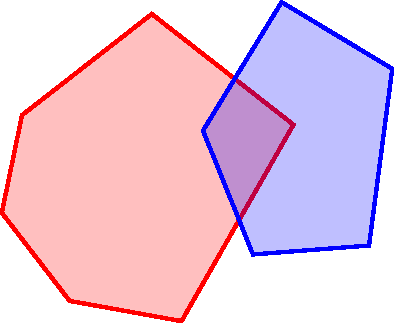
\includegraphics[scale=0.5]{intersections/intersection_simple.pdf}
	  \subcaption{Simple intersection}
	  \label{fig:intersection_simple}
	\end{subfigure}
	\begin{subfigure}[b]{0.4\linewidth}
	  \centering
	  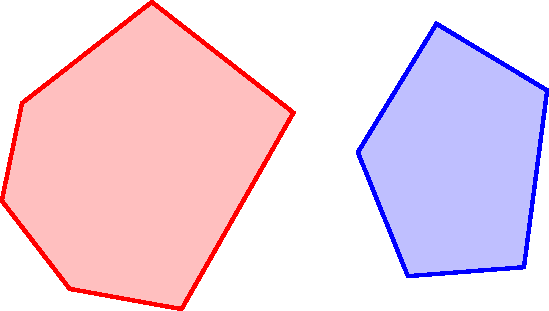
\includegraphics[scale=0.5]{intersections/intersection_none.pdf}
	  \subcaption{No intersection}
	  \label{fig:intersection_none}
	\end{subfigure}
	\begin{subfigure}[b]{0.3\linewidth}
	  \centering
	  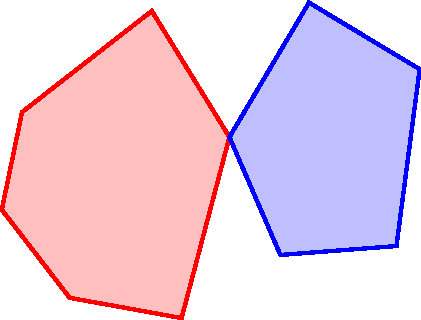
\includegraphics[scale=0.5]{intersections/intersection_point.pdf}
	  \subcaption{Point intersection}
	  \label{fig:intersection_point}
	\end{subfigure}
	\begin{subfigure}[b]{0.3\linewidth}
	  \centering
	  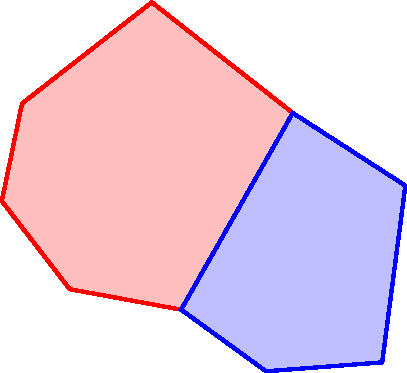
\includegraphics[scale=0.5]{intersections/intersection_line.pdf}
	  \subcaption{Line intersection}
	  \label{fig:intersection_line}
	\end{subfigure}
	\begin{subfigure}[b]{0.3\linewidth}
	  \centering
	  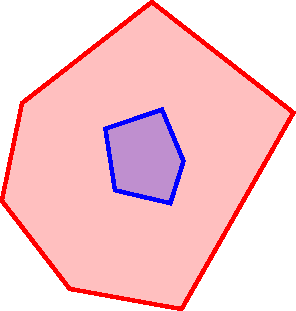
\includegraphics[scale=0.5]{intersections/intersection_inside.pdf}
	  \subcaption{Polygon inside intersection}
	  \label{fig:intersection_inside}
	\end{subfigure}
	\begin{subfigure}[b]{0.3\linewidth}
	  \centering
	  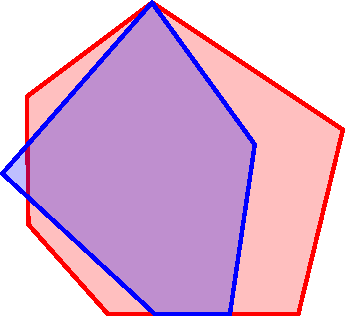
\includegraphics[scale=0.5]{intersections/intersection_fun.pdf}
	  \subcaption{Complex intersection}
	  \label{fig:intersection_fun}
	\end{subfigure}
\caption{Intersections}
\label{fig:intersections}
\end{figure}

As can be seen in figure \ref{fig:intersections}, convex polygon intersections can produce not only empty
and full convex polygons, but also 'degenerate' polygons like points and lines.
Furthermore, there are cases like the polygon being fuly contained inside the
other polygons.

In order for an implementation to be geometrically robust,
all cases (including, but not limited to, the above) must be handled correctly.
This is not trivial, especially if the algorithm used must be efficient.

The algorithm and implementation is sought to be linear in the total number
of points of the intersecting polygons. It is based on a robust variation of the algorithm outlined at
\url{http://www-cgrl.cs.mcgill.ca/~godfried/teaching/cg-projects/97/Plante/CompGeomProject-EPlante/algorithm.html}.

The algorithm is split into several cases, depending on whether the case is Polygon v. Polygon, Polygon v. Line,
Line v. Line, etc. All cases apart from Polygon v. Polygon are somewhat simple, so only Polygon v. Polygon will
be treated here.

The basis of the algorithm is first to find all collision segments, ie. the pairs of directed line segments
of the polygons that collide in at least one point (if they are collinear, they might collide along multiple points).
These collision segments are found through an algorithm based on rotating calipers.
Rotating calipers help find the pocket lids of the algorithm, as well as cases such as collinear collisions.

Once the collision segments have been found in order, they are traversed in order. For each collision segment,
it must be true that one (or both, in which case one is chosen arbitrarily) of the polygons is part of the
intersecting polygon, up until the next collision segment. All the collision segments are followed,
and the result is the convex intersection.

There are several exceptions. If there are no collision segments found, it means that no two line segments
from each polygon cross, meaning that either one polygon is contained in the other, or the polygons
have no overlap. Other examples of cases include where the intersection consists of a single point, or a single line,
in which the involved collision segments and neighbour directed line segments have specific relations.
In the original development, 30 different cases for how collision segments could collide, what it meant and
how to handle were found (handling either means following one polygon or the other, or an exceptional case resulting
in something like a point or a line). This was boiled down to 18 different cases due to common traits and handlings.
These 30 cases should cover all possibilities, helping the robustness of the algorithm.

The big advantage to this relatively complicated algorithm is that it is efficient.
Using the rotating calipers take linear time, and constructing the intersecting polygon from
the collision segments take linear time as well. Assuming that the implementation
has been implemented correctly and efficiently, that means that polygon intersection overall
should take linear time in the number of polygon points.

In regards to efficiency, while it shouldn't be a common problem, convex polygons with many
points may have degraded performance. However, given the very low efficiency of checking images,
a precise convex hull with many points for an image is generally better than a less precise convex hull
with fewer points for an image (of course, if the precisions are the same, the convex hull with the lower
point count should be chosen). For collision primitives with pure convex hulls, ie. no backing images,
trading precision for efficiency in the convex polygon is more likely to be desirable.

